\begin{figure}[h!]
    \centering
    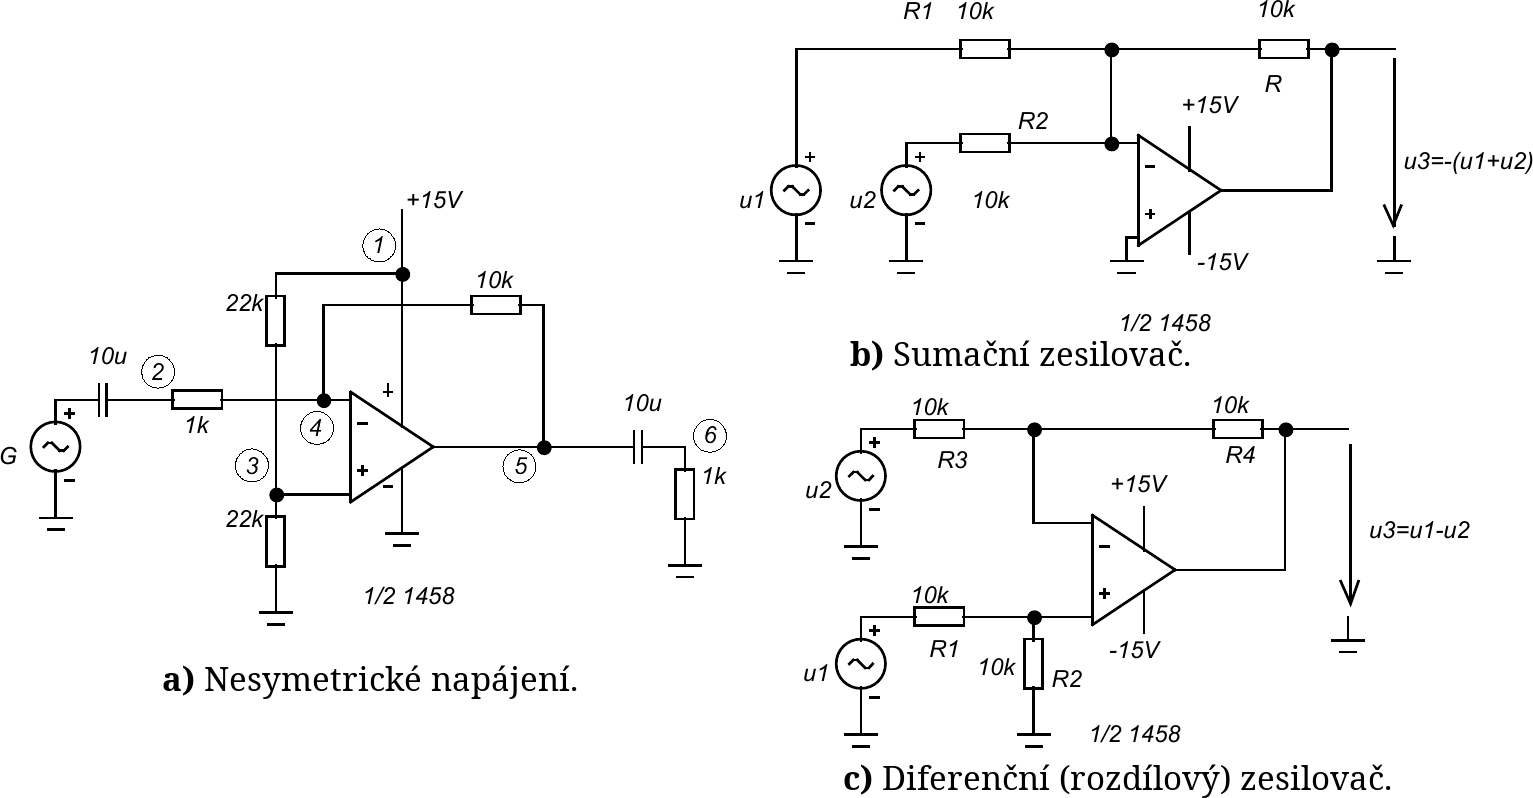
\includegraphics[width=\textwidth]{schema.png}
    \centering
    \caption{Schémata zapojení -- a) jednocestný usměrňovač, b) dvoucestný usměrňovač, c) dvoucestný usměrňovač s minimem přesných součástek.}
    \label{fig:schema}
\end{figure}



\subsection{Funkce jednotlivých zapojení}

    Operační zesilovač s OZ má za úkol překonat nedostatky, které má zapojení pouze s diodami, které díky svému prahovému napětí nedokáží usměrňovat velmi malá napětí. 
    
    Zapojení 1a) je jednocestný usměrňovač, kdy je vždy přes jednu diodu uzavřená záporná zpětná vazba a druhá dioda je uzavřená. Na výstupu je pak signál jednocestně usměrněný a invertovaný. 
    
    Zapojení 1b) pak tento signál zdvojnásobí a sečte s původním vstupním signálem, ve výsledku tedy původní záporné půlvlny zůstanou a kladné po sečtení odpovídají opět záporným. Výsledkem je tedy dvoucestně usměrněný invertovaný signál. 
    Nevýhodou tohoto zapojení je nutnost použít dva co nejshodnější odpory a k nim jeden, který odpovídá hodnotu přesně polovině, při nedodržení nebudou na výstupu půlvlny stejně velké, toto značně zdražuje zapojení. 

    Tento problém se snaží řešit zapojení 1c), kdy pro správnou funkci stačí jedna dvojice přesných odporů \( R_2\) a \(R_3\). Záporná zpětná vazba prvního OZ je vždy uzavřena přes druhý OZ, díky diodám je ale cesta zpětné vazby jiná pro kladný a pro záporný signál, takže ve výsledku je na výstupu druhého OZ signál vždy kladný, neboli dvoucestně usměrněný.   